\documentclass[12pt]{article}
\usepackage[utf8]{inputenc}
\usepackage{amsmath}
\usepackage{amsthm}
\usepackage{amsfonts}
\usepackage{amssymb}
\usepackage{tikz}
\usepackage{pgfplots}
\usepackage{fancyhdr}
\usepackage{enumitem}
\usepackage{hyperref}
\usepackage{dsfont}
\usepackage[ruled,vlined]{algorithm2e}
\usetikzlibrary{intersections, patterns, decorations, automata,positioning,trees,calc}
\pgfplotsset{compat=newest}

\topmargin=-0.45in
\evensidemargin=0in
\oddsidemargin=0in
\textwidth=6.5in
\textheight=9.0in
\headsep=0.25in

\title{Relaxations of the Maximum Cut Problem}
\author{Demetrios V. Papazaharias, Carter Mann, Luca Wrabetz\\ \small Department of Industrial and Systems Engineering \\
\small University at Buffalo, Bell Hall, Buffalo, New York, 14260\\\small $\lbrace \text{dvpapaza, cjmann3, lucawrab}\rbrace$@buffalo.edu}
\date{December 2019}

\theoremstyle{plain}
\newtheorem{prop}{Proposition}
\newtheorem{theorem}{Theorem}
\newtheorem{claim}{Claim}
\theoremstyle{definition}
\newtheorem{defn}{Definition}
\newcommand{\matr}[1]{\mathbf{#1}}

\tikzstyle{vertex}=[circle, draw, inner sep=0pt, minimum size=6pt]
\newcommand{\vertex}{\node[vertex]}

\DeclareMathOperator*{\argmax}{arg\,max}
\DeclareMathOperator*{\argmin}{arg\,min}
\newcommand{\norm}[1]{\left\lVert#1\right\rVert}
\begin{document}
\maketitle
\begin{abstract}
    Maximum cut is a classic NP-Hard problem in combinatorial optimization. In this work we present several relaxations for the maximum cut problem. 
\end{abstract}

\clearpage
\section{Introduction}\label{sec:Introduction}
The maximum cut problem (maxcut) is a classical problem in combinatorial optimization in which we are given a graph $G = (V, E)$, with node set $V = \lbrace 1,...,n \rbrace$ and edge set $E = \lbrace i, j \rbrace \subseteq \binom{V}{2}$. We are also given, for each edge $\{i, j\} \in E$, a non-negative weight $w_{ij}$ . The maxcut problem consists in determining a subset of $S \subseteq V$ nodes for which the sum of the weights of the edges that cross from $S$ to its complement $\bar{S}$ (i.e., the weight of the edges in the cut $(S, \bar{S})$ is maximized. In this particular case, we are assuming that the edges are undirected; however, this problem can be easily generalized to the directed case.

Unlike the minimization variant to this problem, which can be solved in polynomial time, the maxcut problem is NP-Hard. Given its nature, the maxcut problem is a highly studied problem in Graph Theory. Although no polynomial algorithm exists to solve maxcut (Unless we discover $P = NP$) a multitude of approximation algorithms and heuristics have been developed in an attempt to solve this problem to a relative level of optimality. One simplistic method is a local search algorithm, which starts with an arbitrary set $S$ and then iteratively either adds or removes an edge, as long as it helps the objective function. A more complex method would be the Goemans and Williamson algorithm, which  combines semi-definite programming and a rounding procedure to produce an approximate solution to the max-cut problem.

In this paper we will focus our attention on IP formulations to the maxcut, along with a variety of relaxations and a heuristic which will help us find upper and lower bounds respectively. In section 2 we will discuss two separate formulations to the maxcut. Section 3 will feature a variety of relaxations to the maxcut, which will help us find upper bounds to our problem.  Section 4 will discuss a heuristic which utilizes two-swap simulated annealing approach to find a sufficient lower bound to our problem.  Section 5 will display the computational analysis for our study, and finally section 6 will be the conclusion to our findings.
\section{Mathematical Formulations}\label{sec:Formulations}
\subsection{Formulation 1}\label{subsec:Formulation1}
In this formulation, we define binary variables $x_{i}$ for each $i \in V$ that indicate whether node $i$ belongs to $S$. we also define the binary variables $y_{ij}$ to indicate whether edge $\lbrace i,j \rbrace$ is part of the cut.
Using these variables, we can formulate this problem as follows:
\begin{align}
     z^* = \max \quad &\sum_{\lbrace i,j\rbrace \in E} w_{ij}y_{ij} \\
     \text{s.t.}\quad &y_{ij} \leq 2 - x_i - x_j,\quad \lbrace i,j \rbrace \in E \\
      &y_{ij} \leq x_i + x_j,\quad \lbrace i,j \rbrace \in E \\
       &y_{ij} \geq x_i - x_j,\quad \lbrace i,j \rbrace \in E \\ 
       &y_{ij} \geq x_j - x_i,\quad \lbrace i,j \rbrace \in E \\ 
       &x_i \in \lbrace 0,1 \rbrace, \quad \quad \quad i \in V \\
        &y_{ij} \in \lbrace 0,1 \rbrace, \quad \lbrace i,j \rbrace \in E
\end{align}
where constraint (2) imposes that if both ends of an edge are in $S$, this edge is not in the cut, (3) imposes that if both ends are in $\bar{S}$, this edge is not in the cut, (4) and (5) impose that if the ends of this edge are in different sets, this edge is in the cut, and (6) and (7) define the domain of the variables. 
\subsection{Formulation 2}\label{subsec:Forulation2}
In this formulation, we define variables $z_i$ for each $i \in V$ to take the value of $-1$ if $i \in S$ and $1$ if $i \notin S$. Using these variables, we can formulate this problem as follows:
\begin{align}
     z^* = \frac{1}{4}\max \sum_{i \in V} \sum_{j \in V} w_{ij} (1 - z_i z_j) \\ st.\quad z_i \in \lbrace -1,1 \rbrace, \quad \quad i \in V 
\end{align}



\section{Relaxations for Max Cut}\label{sec:Relaxations}

In this section we propose several relaxations, other than the linear programming relaxation for Max Cut. We restrict the contents of this sections to algorithms and necessary proofs for computing each bound. We postpone discussion of results, selected parameters and implementation for the computational study in Section 5.

\subsection{Eigenvalue Relaxation}\label{subsec:Eigenvalue}

We define the Laplacian of graph $G$ as the matrix $L(G) = D(G) - A(G)$ such that $D(G)_{ii} = \sum_{j \in V: \lbrace i,j \rbrace \in E} w_{ij}$, $D(G)_{ij} = 0$ for $i,j \in V, i \neq j$, and $A(G)_{ii} = 0$ for $i \in V$ and $A(G)_{ij} = w_{ij}$ for $i,j \in V$ such that $i \neq j$. The Laplacian is well studied in spectral graph theory. In this work we will utilize $L(G)$ in order to compute the upper bound for Max Cut.

\begin{prop}
The optimal value of $z^*$ in the max cut problem defined on graph $G=(V,E)$ satisfies
\[
    z^* \leq z^{ev} := \dfrac{n}{4} \lambda_{max}(L(G))
\]
\end{prop}

\begin{proof}
    Consider the maximization problem 
    \[
    \max\lbrace \mathbf{z}^\top L(G) \mathbf{z}\,|\,\mathbf{z} \in \lbrace -1,1 \rbrace^n  \rbrace
    \]
    Since $L(G) = D(G) - A(G)$, then $L(G)_{ii} = \sum_{j\in V} w_{ij}$ for $i \in V$ and $L(G)_{ij} = -w_{ij}$ for $i,j \in V$ such that $i \neq j$. We expand the objective function and obtain
    \[
        \max_{\mathbf{z} \in \lbrace -1,1 \rbrace} \sum_{i \in V}\sum_{j \in V} w_{ij} z_i z_i - \sum_{i \in V}\sum_{j \in V} w_{ij}z_i z_j
    \]
    Furthermore,
    \[
        \max_{\mathbf{z} \in \lbrace -1,1 \rbrace} \sum_{i \in V} \sum_{j \in V} w_{ij} (z_i z_i - z_i z_j) 
    \]
    Since $z_i \in \lbrace -1, 1 \rbrace$ then $z_i z_i=1$, we can simplify the objective function to
    \[
        \max_{\mathbf{z} \in \lbrace -1,1 \rbrace} \sum_{i \in V} \sum_{j \in V} w_{ij} (1- z_i z_j)
    \]
    From the previous section we saw an almost identical formulation for max cut. The only difference being a multiplier of $\frac{1}{4}$. Let $z^*$ represent the optimal solution for max cut
    \begin{equation}\label{eq:optimalZLaplace}
        z^* = \frac{1}{4} \max \lbrace \mathbf{z}^\top L(G) \mathbf{z} \,|\, \mathbf{z} \in \lbrace -1,1 \rbrace^n \rbrace
    \end{equation}
    Taking the continuous relaxation of (\ref{eq:optimalZLaplace}), namely $z_i \in \left[-1,1 \right]$ for $i \in V$, is equivalent to maximizing
    over the norm infinity, $\norm{\mathbf{z}}_\infty \leq 1$. We can relax this further by maximizing over a ball of radius $\sqrt{n}$. In other words,
    our region is now defined where $\norm{\mathbf{z}} \leq \sqrt{n}$. 
    \begin{equation}
    z^* \leq \frac{1}{4} \max \lbrace \mathbf{z}^\top L(G) \mathbf{z} \,|\, \mathbf{z} \leq \sqrt{n} \rbrace
    \end{equation}    
    We can define our problem over the unit ball with a simple transformation. Let $\norm{\mathbf{z}} = \sqrt{n} \mathbf{x}$ and
    we now have
    \begin{equation}
        z^* \leq \frac{n}{4} \max \lbrace \mathbf{x}^\top L(G) \mathbf{x} \,|\, \norm{\mathbf{x}} \leq 1 \rbrace
    \end{equation}  
    Since for any symmetric matrix $\mathbf{A}$, $\max\lbrace \mathbf{x}^\top \mathbf{A} \mathbf{x}\,|\, \norm{\mathbf{x}} \leq 1 \rbrace = \lambda_{\max(\mathbf{A})}$ 
    and $L(G)$ is symmetric, then we have 
    \begin{equation}
    z^* \leq z^{ev} := \dfrac{n}{4} \lambda_{max}(L(G))
    \end{equation}
\end{proof}



\begin{prop}
    The optimal value of $z^*$ in the max cut problem defined on graph $G=(V,E)$ satisfies
    \[
        z^* \leq z^{ev} := - \frac{1}{4}\sum_{i=1}^n u_i + \dfrac{n}{4} \lambda_{max}(L(G) + diag(\mathbf{u}))
    \]
    for all $\mathbf{u} \in \mathbb{R}^n$
\end{prop}

\begin{proof}
    Consider the maximization problem
    \begin{equation}\label{eq:propopt2}
        \max\lbrace \mathbf{z}^\top (L(G) + diag(\mathbf{u})) \mathbf{z} | \mathbf{z} \in \lbrace -1,1\rbrace \rbrace
    \end{equation}
   
    From the previous proof, we perform a similar technique to (\ref{eq:propopt2}) to obtain the following optimization problem 
    \[
    \max_{\mathbf{z} \in \lbrace -1,1 \rbrace} \sum_{i \in V}\left(\sum_{j \in V} w_{ij} + u_i \right) z_i z_i - \sum_{i \in V}\sum_{j \in V} w_{ij}z_i z_j
    \] 
    Rearranging terms and using the fact that $z_i z_i = 1$,
    \begin{equation}
        \max_{\mathbf{z} \in \lbrace -1, 1\rbrace} \sum_{i = 1}^n \sum_{j=1}^n w_{ij} (1 - z_i z_j) + \sum_{i = 1} u_i \label{eq:eig2}
    \end{equation}
    Which is closely related to the objective function in our prevoius formulation. We obtain the following relationship between (\ref{eq:eig2}) and $z^*$:
    \[
      z^* = \frac{1}{4} \max\lbrace \mathbf{z}^\top (L(G) + diag(\mathbf{u})) \mathbf{z} \,|\, \mathbf{z} \in \lbrace -1,1\rbrace \rbrace - \frac{1}{4}\sum_{i=1}^n u_i   
    \]
    We repeat the process from the previous proof of relaxing the variables so that they are continuous and then further relaxing this problem onto a ball of radius $\sqrt{n}$.
    \[
        z^* \leq \frac{1}{4} \max\lbrace \mathbf{z}^\top (L(G) + diag(\mathbf{u})) \mathbf{z} \,|\, \norm{\mathbf{z}} \leq \sqrt{n} \rbrace - \frac{1}{4}\sum_{i=1}^n u_i
    \]
    Let $\mathbf{z} = \sqrt{n} \mathbf{x}$. 
    \[
        z^* \leq \frac{n}{4} \max\lbrace \mathbf{x}^\top (L(G) + diag(\mathbf{u})) \mathbf{x} \,|\, \norm{\mathbf{x}} \leq 1\rbrace - \frac{1}{4}\sum_{i=1}^n u_i
    \]
    Finally, we obtain the inequality
    \begin{equation}
        z^* \leq z^{ev}(\mathbf{u}) = -\frac{1}{4}\sum_{i=1}^n u_i + \dfrac{n}{4} \lambda_{max}(L(G) + diag(\mathbf{u}))
    \end{equation}
\end{proof}
    
\subsection{Lagrangian Dual}\label{subsec:LDbound}

In the previous section we have proved several upper bounds on max cut based on the Laplace $L(G)$, including one which changes of the diagonal of $L(G)$ with some vector $\mathbf{u} \in \mathbb{R}^n$. In this section we will
compute the Lagrangian dual bound of maximum cut, which corresponds to the values of $\mathbf{u}$ such that $z^{ev}(\mathbf{u})$ is minimized.
\[
    z^{LD} = \min\Bigg\lbrace -\frac{1}{4}\sum_{i=1}^n u_i + \dfrac{n}{4} \lambda_{max}(L(G) + diag(\mathbf{u})) \,\Bigg|\, \mathbf{u} \in \mathbb{R}^n \Bigg\rbrace
\]
Consider the gradient of our objective function, $\nabla z^{ev}(\mathbf{u})$. In order to compute $\nabla \lambda_{max}(L(G) + diag(\mathbf{u}))$ we first use the fact that $L(G) + diag(\mathbf{u})$ is a symmetric square matrix and therefore $\lambda_{max}(L(G) + diag(\mathbf{u})) = \max\lbrace \mathbf{x}^\top (L(G) + diag(\mathbf{u})) \mathbf{x} \,|\,\norm{\mathbf{x}} \leq 1\rbrace$. This optimization problem can further be expanaded to
\[
\max_{\norm{\mathbf{x}} \leq 1} \sum_{i \in V} \left(\sum_{j \in V} w_{ij} + u_i \right) x_i x_i - \sum_{i \in V} \sum_{j\in V} w_{ij}x_i x_j 
\]
We can see that this objective value is maximized for $x_k = 1$ where $k = \argmax_i\large\lbrace \sum_{j \in V} w_{ij} + u_i \, |\, \sum_{j \in V} w_{ij} + u_i  > 0\large\rbrace$, and $x_i = 0$ for $i \in V \setminus \lbrace k \rbrace$. If there exists no positive value of  $\sum_{j \in V} w_{ij} + u_i $ then the objective function is maximized for $\mathbf{x} = \mathbf{0}$. Therefore, $\nabla \lambda_{max}(L(G) + diag(\mathbf{u})) = e_k$ if $ \lambda_{max}(L(G) + diag(\mathbf{u}))  \geq 0$ and $\mathbf{0}$ otherwise and  $\nabla z^{ev}(\mathbf{u})$ can be computed as
\[
 \nabla z^{ev}(\mathbf{u})_k = \begin{cases}
 \frac{n-1}{4} \quad& \text{if }k =\argmax_i\Big\lbrace \sum_{j \in V} w_{ij} + u_i  \,\Big|\, \sum_{j \in V} w_{ij} + u_i  > 0\Big\rbrace\\
 -\frac{1}{4} \quad&\text{otherwise}
 \end{cases}
\]
\subsubsection{Subgradient Algorithm}\label{subsubsec:Subgradient}

We implement the following subgradient algorithm in order to compute $z^{LD}$. We postpone details on our implementation decisions such as stopping criteria, initial solutions and choice of sequence $h_k$ for a later section.

\vspace{0.2cm}

\begin{algorithm}[H]
	\SetAlgoLined
	\KwResult{Computes the Lagrangian dual bound $z^{LD}$}
	Select an initial solution $\mathbf{u}_0$ and appropriate sequence $\lbrace h_k \rbrace_{k=0}^\infty$\;
	\For{$k \geq 0$}{
		Compute $z^{ev}(\mathbf{u})$ and $\nabla z^{ev}(\mathbf{u})$\;
		$\mathbf{u}_{k+1} \gets \mathbf{u}_k - h_k \frac{\nabla z^{ev}(\mathbf{u})}{ \norm{\nabla z^{ev}(\mathbf{u})}}$\;
	}
	\caption{Subgradient Algorithm for MaxCut}
\end{algorithm}

\subsection{Semi Definite Relaxation}\label{subsec:SDRelax}
The semi-definite relaxation of formulation 2 is expressed as follows: 

\begin{align}
    z^{*} = \frac{1}{4} \max \quad & \sum_{i \in V} \sum_{j \in V} w_{ij}(1-Y_{ij}) \\
    \text{s.t} \quad & Y_{ii} = 1, \quad i \in V\\
     & \matr{Y} \succeq 0
\end{align}

The formulation is relaxed by introducing the matrix $\matr{Y}$. The elements $Y_{ij}$ of this matrix correspond to the multiplication of the decision variables $z_{i}$ and $z_{j}$ from the original formulation. Additionally, the variables are relaxed such that $Y_{ij} \in \mathbb{R}$. Constraint (18) enforces the fact that $z_{i} = z_{i}$ from the original formulation, as the multiplication of 1 and 1 or -1 and -1 results in 1. This also makes sense conceptually, as the same node can't be in two different sides of the cut. Thus, we will maintain the diagonal of the matrix $\matr{Y}$ fixed during the solution of this formulation. Constraint (19), forces the values of $Y_{ij}$ variables to stay between -1 and 1, and ultimately converge close to either 1 or -1 in feasible solutions. 

To solve the formulation, we implement the ellipsoid algorithm. The algorithm is generally efficient and effective for convex problems, such as the relaxed formulation. However, we know that its nature causes it to be slow in practice in many cases, as it can iterate between infeasible and feasible solutions for a large number of steps. We will discuss this further in our computational analysis. 

The ellipsoid algorithm relies on affine transformations between a unit "ball", $B(y_{k},1)$, and ellipsoids $E(y_{k}, \matr{H_{k}})$. Notice, that the value $\mathbf{y}$ is the current proposed solution at iteration k. Ultimately, the algorithm works on each iteration and its current $\mathbf{y_{k}}$ in the space of $B(0, 1)$, and transforms new solutions in the ellipsoid space to continually shrink and shift the ellipsoids and converge to better, feasible solutions. At each iteration, if the current solution is infeasible, a separating cut is added to move the next $\mathbf{y_{k}}$ towards feasibility: if it is not PSD, the eigenvector associated with the most violating eigenvalue is used to calculate the direction to move in for $y_{k+1}$. If the solution is feasible, we move in the direction of the objective function's gradient.

Suppose we define the feasible region for our semi-definite relaxation to be the set $K = \{y_{ij} : Y_{ii} = 1, Y_{ij} = Y_{ji}, Y \succeq 0, i \in V, j \in V\}$. In reality, when the algorithm is implement, we only need to maintain a vector of variables $y_{i}, i \in V$, since the constraints $Y_{ii} = 1, Y_{ij} = Y_{ji}$ can be trivially disgarded without loss of generality, and the matrix $\matr{Y}$ can be constructed and converted back to the list $\mathbf{y}$ at every iteration. The algorithm is initialized by finding a value $R \in \mathbb{R}$ such that $K \subseteq B(0, R)$, and thus, our initial solution, $\mathbf{y_{0}}$, is the zero vector, and $\matr{Y}$ is the identity. Thus, we wish for our initial ellipsoid to be $B(0, R)$, so we initialize $\matr{H_{0}}$ to be $R^{2}\matr{Y}$. Thus, we iterate over the algorithm described earlier as follows: \\

\vspace{0.25cm}


\begin{algorithm}[H]
    \SetAlgoLined
    \KwResult{Solution to Semi-Definite Relaxation}
    $R$ $\gets$ $2n$\;
    $\matr{Y_{0}}$ $\gets$ identity\;
    $\mathbf{y_{0}} \gets \mathbf{0}$ \;
    $\matr{H_{0}}$ $\gets$ $R^{2}\matr{Y}$\;
    $\mathbf{g}$ $\gets \nabla z$\;
    $\epsilon$ $\gets$ 0.001\;
    $change$ $\gets$ 100\;
    $k \gets$ 0\;
    \While{change $>$ $\epsilon$}{
        \eIf{$\matr{Y_{k}} \succeq 0$}{
            $\mathbf{y_{k+1}}$ $\gets$ ellipsoidshift($\matr{Y_{k}}$, $\mathbf{g}$, $\matr{H_{k}}$) \;
            $\matr{H_{k+1}}$ $\gets$ newH($\matr{Y_{k}}$, $\mathbf{g}$, $\matr{H_{k}}$) \;
            }{
            $\overline{g} \gets$ separatingcut(min\_eigenvector) \;
            $\mathbf{y_{k+1}}$ $\gets$ ellipsoidshift($\matr{Y_{k}}$, $\overline{\mathbf{g}}$, $\matr{H_{k}}$) \;
            $\matr{H_{k+1}}$ $\gets$ newH($\matr{Y_{k}}$, $\overline{\mathbf{g}}$, $\matr{H_{k}}$) \;
            }
        $k$ $\gets$ $k+1$ \;
        $change$ $\gets$ $||\mathbf{y_{k+1}} - \mathbf{y_{k}}||$ \;
    }
    return $\mathbf{y}$ \;
	\caption{Ellipsoid Algorithm for MaxCut.}
\end{algorithm} 

The side funtions ellipsoid shift, and new H, are implementations of the closed-form matrix operations from the project guidelines. The vector $\mathbf{g}$ remains constant, and is the gradient of the objective function. This is the direction we want to move in when our solution is already feasible. $\overline{\mathbf{g}}$ is calculated by taking the gradient of the most violating eigenvector in the function separatingcut.

\section{Heuristic Solution}

In this section we introduce a 2-swap simulated annealing heuristic to compute good feasible solutions for Max Cut. The outline of this sections is as follows

\subsection{Greedy Initial Solution}

In order to obtain an initial feasible solution for our heuristic we first sort the edges by weight in descending order. Then. for each edge $\lbrace i,j \rbrace \in E$ we check which set $i$ and $j$ are assigned to. If either of the endpoints are not assigned to $S$ or $\overline{S}$ , without loss of generality say $j$, the place $j$ into the opposite set of $i$ and add $\lbrace i,j \rbrace$ to the cut. If both nodes are unassigned then $S \gets S \cup \lbrace i \rbrace$ and $\overline{S} \gets \overline{S} \cup \lbrace j \rbrace$ and we add $\lbrace i,j \rbrace$ to the cut. Otherwise, we cannot place $\lbrace i,j \rbrace$ in the cut and maintain a feasible solution. This construction can be completed in $O(m \log m)$, where the dominant procedure is the sorting of $E$. In addition, this procedure will place every vertex $v$ into $S$ or $\overline{S}$, unless $v$ has degree 0. In that case we can remove $v$ from $V$ and it does not effect the solution.

\subsection{2-Swap Procedure}

At each iteration of our heuristic we will randomly select one vertex $i \in V$ and another vertex $j$ such that $j \in \overline{S}$ if $i \in S$ and vice-versa.  We will navigate through the solution space of Max Cut by swapping the sets which $i$ and $j$ belong to. In order to efficiently compute the change in the objective function from this swap we will only check the neighbors of $i$ and $j$. Suppose $i \in S$ and $j \in \overline{S}$, for each $k \in N(i)$ such that $k \in S$, we add $w_{ik}$ to the current objective value as $i$ will belong to the complement of $S$ after the swap. Conversely, for each $\ell \in \overline{S}$ we subtract $w_{i\ell}$ from the current objective. However, we must account for the case when $j \in N(i)$. Since $j$ was originally in $\overline{S}$, $w_{ij}$ was subtracted from the current solution. However, $j$ will be placed into $S$ after the swap, we must correct this by adding $w_{ij}$ to the objective value. We repeat this procedure for $j$ and obtain the potential benefit of swapping $i$ and $j$. This benefit can be computed in $O(m)$ time. 

\begin{figure}[h]
	\centering
	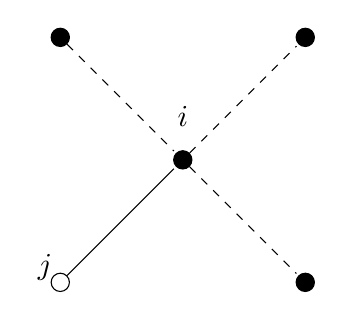
\begin{tikzpicture}[shorten >=1pt,node distance=2cm,on grid,auto,scale=1.1, every node/.style={transform shape}]
	\node[vertex, fill] (u) {};
	\node[vertex, fill, above left of= u] (u1) {};
	\node[vertex,  below left of= u] (v) {};
	\node[vertex, fill,  below right of= u] (u2) {};
	\node[vertex, fill, above right of= u] (w) {};
	\node[above=0.5cm of u] (uname){$i$};
	\node[above left=0.25cm of v] (vname){$j$};
	\path[-]
	(v) edge (u);
	\path[-,dashed]
	(u1) edge (u)
	(u) edge (u2)
	(u) edge (w);
	\end{tikzpicture}
	\hspace{2cm}
	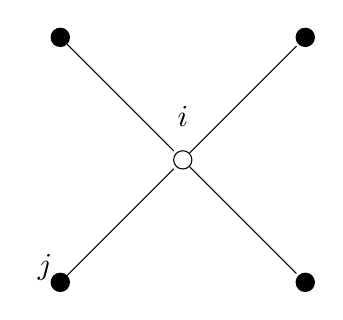
\begin{tikzpicture}[shorten >=1pt,node distance=2cm,on grid,auto,scale=1.1, every node/.style={transform shape}]
	\node[vertex] (u) {};
	\node[vertex, fill, above left of= u] (u1) {};
	\node[vertex,fill,   below left of= u] (v) {};
	\node[vertex, fill,  below right of= u] (u2) {};
	\node[vertex, fill, above right of= u] (w) {};
	\node[above=0.5cm of u] (uname){$i$};
	\node[above left=0.25cm of v] (vname){$j$};
	\path[-]
	(v) edge (u);
	\path[-]
	(u1) edge (u)
	(u) edge (u2)
	(u) edge (w);
	\end{tikzpicture}
	\caption{2-swap procedure for Max Cut}
\end{figure}

\subsection{Simulated Annealing}

Simulated Annealing is a neighborhood based search method which is improving but occasionally allows switching to worse solutions in order to escape local minima. The motivation from this method came from the physical process of annealing metal, in which the metal is heated and cooled slowly in order to create a stronger material. The parameters for this algorithm include:

\begin{enumerate}
	\item  An initial temperature $T_0$, which is typically computed in relation to the worst possible neighboring solution
	\item A temperature length $T_L$ which represents how many neighboring solution we will check at each temperature
	\item A cooling function which decreases the temperature for the next iteration
	\item A stopping criteria, which in our case will be a threshold on temperature
\end{enumerate}

At each iteration a random neighboring solution is selected,  a potential 2-swap in this case, and the difference in objective between the current and new solution is computed. If the new solution is an improvement, it is always accepted. If the new solution is worse, then we accept the solution based on a probability function of the magnitude in the objective value change and the current temperature.

\vspace{0.25cm}

\begin{algorithm}[H]
	\SetAlgoLined
	\KwResult{Feasible solution for Max Cut}
	Construct initial greedy solution $\mathbf{z}$ and select appropriate  $\alpha, \Delta_{accept}, T_{stop}, T_{L}$\;
	$z_{best} \gets z$\;
	$T_{now} \gets -\frac{\Delta_{max}}{\log -\Delta_{accept}}$\;
	\While{$T_{now} > T_{stop}$}{
	\For{$t \in T_{L}$}{
		Select $i,j$ from opposite components and compute $\Delta(i,j)$\;
		\eIf{$\Delta(i,j) > 0$}{
			Swap($i,j$)\;
			$z = z + \Delta(i,j)$
		}{
			$q \gets $ random($0,1$)\;
			\If{$\exp\lbrace \Delta(i,j) / T_{now}\rbrace > q$}{
				Swap($i,j$)\;
				$z = z + \Delta(i,j)$
			}
		}
		\If{$z > z_{best}$}{
		$z_{best} \gets z$
	}
		}
		$T_{now} \gets \alpha T_{now}$\;
	}
	\caption{Simulated Annealing for Max Cut}
\end{algorithm}

\section{Computational Study}

In this section we present all computational results for each method discussed on 92 randomly generated weighted graphs. These instances consisted of thirty graphs with $n \in \lbrace 10, 15, 20\rbrace$ and expected edge density $d \in \lbrace 0.2, 0.5, 0.8 \rbrace$, as well as a graph with $n=50, d = 0.8$ and $n= 100, d= 0.2$. All algorithms were implemented in Python. Gurobi Optimizer 9.0 was used to solve all 0-1 programming formulations. All numerical experiments were conducted on a Linux Manjaro OS with Intel 2 Core i3-2100$@$1.6 GHz and 8-GB RAM.

\subsection{Implementation Decisions}

In this section we provide all of our implementation decisions and selected parameters for each method. 

\subsubsection{Integer Program}

In this section we introduce the results of the integer program. Each instance was given a time limit of 600 seconds. All instances of such that $n \leq 20$ reached its optimal solution within this time where as the 50 and 100 node instance did not. 


\subsubsection{Lagrangian Dual Relaxation}

In our computational study the selected sequence $h_k = M \rho^k$ with $M = 2n$ and $\rho = 0.98$ produced the overall best bound for most instances.

\subsubsection{Ellipsoid Algorithm} 

For our implementation of the Ellipsoid algorithm we made several decisions regarding the initial solution and stopping criteria. Our initial solution $\mathbf{y}_k =\mathbf{0}$, in other words we begin with $\mathbf{Y}$ as the identity matrix. In order to select an initial $R$ we consider the maximum distance between feasible solutions of $Y$. Consider the feasible solutions $Y_{ij} = 1$ for $i,j \in V$ and $Y_{ij} = -1$ for $i,j \in V$ such that $i \neq j$. The distance between these solutions can be computed as the element wise Euclidean distance. Since $\mathbf{Y} \in \mathbb{R}^{n \times n}$, the distance can be no larger than $2n$. As a result, we set $R = 2n$ for our algorithm.

Since the Ellipsoid algorithm can move to worse solutions throughout the algorithm we will select the $\norm{\mathbf{y}_{k+1} - \mathbf{y}_k} < \epsilon$ as our stopping criteria. We set $\epsilon = 0.001$ as it provided us the best trade off between computation time and a feasible bound.

\subsubsection{Simulated Annealing}

\section{Conclusion}
\end{document}
